\chapter[Datos]{Datos}
\label{Chap2}

Para este proyecto disponemos de los siguientes datos obtenidos de distintas páginas web:
\begin{itemize}
	\item Nivel (m)
	\item Caudal ($m^3/s$)
	\item Precipitación (mm)
	\item Temperatura (ºC)
	\item Humedad (\%)
	\item Radiación ($W/m^2$)
\end{itemize}
A su vez, se dispone de la fecha y hora en la que se hicieron la lectura de los datos, junto con los códigos y coordenadas de las estaciones sobre las cuales obtenemos los datos.

\section{Aemet}
Como se ve en la imagen \ref{fig:ej3}, dentro de la web podemos encontrar de forma accesible múltiples datos relacionados con la meteorología tomados cada hora, de los cuales seleccionaremos únicamente temperatura, precipitación y humedad, puesto que los datos relacionados con el viento no son tan relevantes para este proyecto.

\begin{figure} [H]
	\centering
	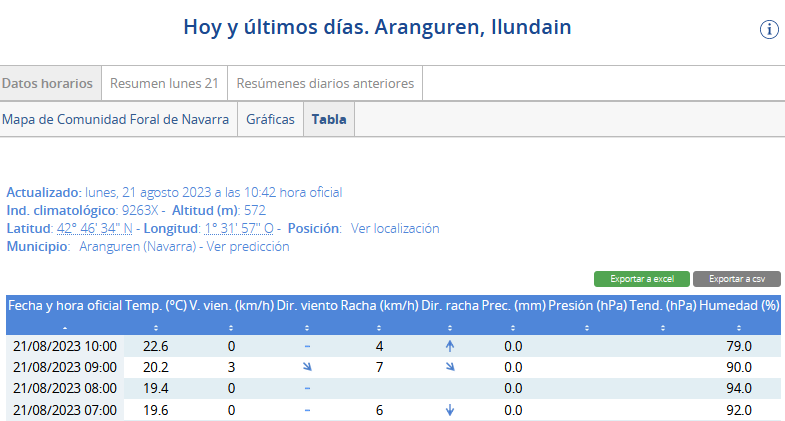
\includegraphics[width=0.7\textwidth]{fig/AemetData.png}
	\caption[Página Aemet de la estación en Aranguren (Navarra)]{Página Datos Aemet}
	\label{fig:ej3}
\end{figure}

Los datos en HTML vienen datos dentro de un elemento tabla \ref{fig:ej20}, lo que facilita su adquisición, tomando todas las filas de esta dentro de elemento tbody. Una vez obtenidas las filas, la forma de lograr los datos deseados seria eligiendo dentro de cada elemento tr los elementos td deseados, puesto que HTML empieza a contar elementos desde el uno (en vez de cero como suele ser común en lenguajes de programación), los td a obtener serian: uno, fecha y hora; dos, temperatura; siete, precipitación; diez, humedad.

\begin{figure} [H]
	\centering
	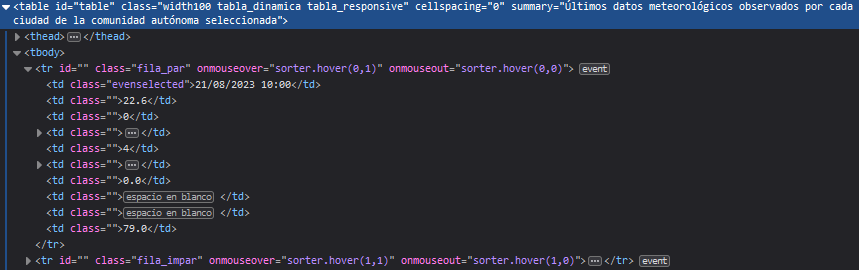
\includegraphics[width=0.7\textwidth]{fig/AemetDataHTML.png}
	\caption[HTML de la tabla de datos de Aemet de la estación en Aranguren (Navarra)]{HTML Tabla Datos Aemet}
	\label{fig:ej20}
\end{figure}

Las coordenadas, dentro de un span, están incluidas en elementos abbr con sus respectivas clases "latitude" y "longitude", haciendo posible su obtención fácilmente mediante los elementos abbr.

\begin{figure} [H]
	\centering
	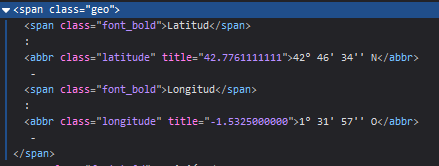
\includegraphics[width=0.7\textwidth]{fig/AemetCoordHTML.png}
	\caption[HTML de las coordenadas de Aemet de la estación en Aranguren (Navarra)]{HTML de las coordenadas en Aemet}
	\label{fig:ej21}
\end{figure}

\section{El Agua en Navarra}
En esta página encontraremos los datos tanto del nivel de los ríos como de su caudal en los últimos 15 días en periodos de 10 minutos, siendo una de las fuentes principales de datos.
\newline
\newline
La sección de aforos en la página \ref{fig:ej4} muestra el mapa de Navarra junto a varias estaciones. Aunque no todas las disponibles en la web, conformando unicamente el grupo de estaciones principales.\newline
\newline
Con el fin de acceder a todas las estaciones disponibles, debemos centrarnos en el mapa de la esquina inferior derecha. Estructurada en 6 regiones, Norte, Arga, Ega, Ebro alto, Ebro bajo y Aragón, por medio de este mapa accedemos a cada región, mostrando el mapa de la región, dando acceso a todas las estaciones en la zona.

\begin{figure} [H]
	\centering
	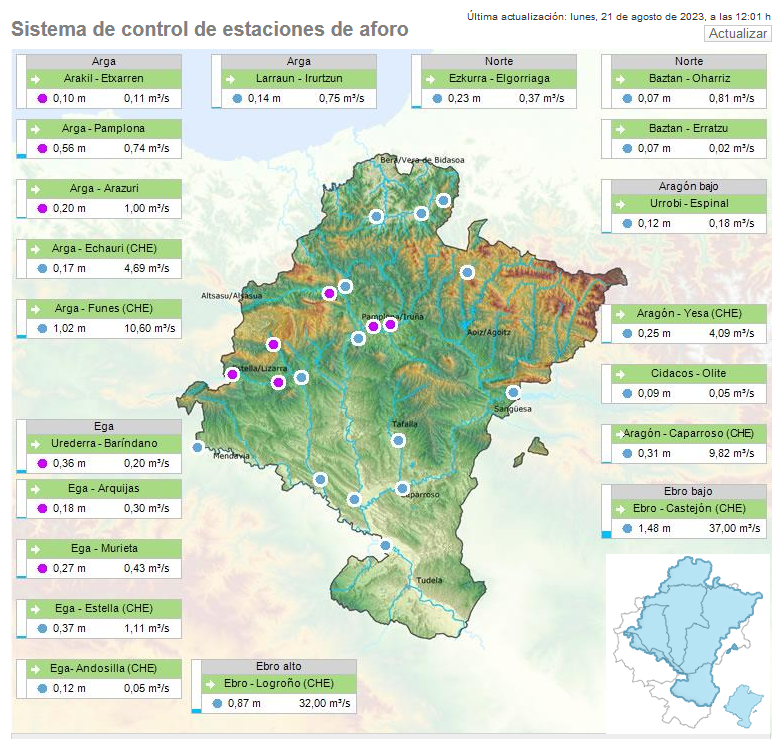
\includegraphics[width=0.7\textwidth]{fig/AguaEnNavarraCode.png}
	\caption[Página principal de aforos de El Agua en Navarra]{Página El Agua en Navarra}
	\label{fig:ej4}
\end{figure}

El HTML del mapa se estructura de la siguiente manera \ref{fig:ej22}, mostrando un par de elementos area por estación, uno con shape "rect", representando las tarjetas que rodean el mapa y otro con shape "circle", siendo los puntos en el mapa. Pulsar sobre cualquiera de ellos es equivalente, aunque posteriormente hagamos uso de los elementos "rect" dentro del código.

\begin{figure} [H]
	\centering
	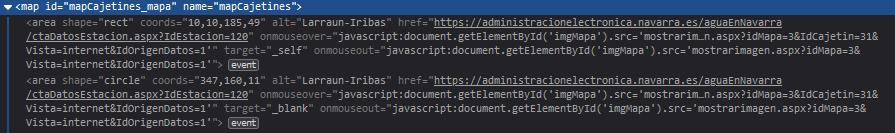
\includegraphics[width=0.7\textwidth]{fig/AguaEnNavarraCodeHTML.png}
	\caption[HTML mapa estaciones de El Agua en Navarra]{HTML mapa estaciones El Agua en Navarra}
	\label{fig:ej22}
\end{figure}

Las paginas de cada estación se muestran así \ref{fig:ej23}.

\begin{figure} [H]
	\centering
	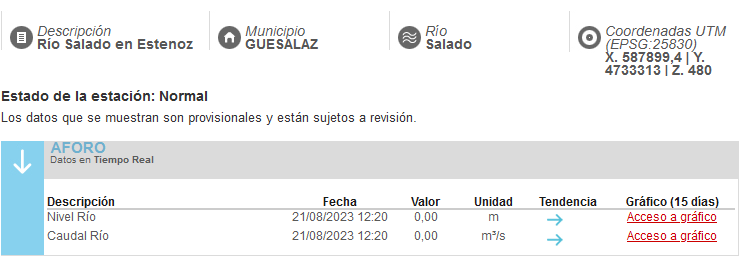
\includegraphics[width=0.7\textwidth]{fig/AguaEnNavarraEstacion.png}
	\caption[Página estación de El Agua en Navarra]{Página estación El Agua en Navarra}
	\label{fig:ej23}
\end{figure}

De ella obtenemos los próximos datos, descripción, municipio, río y coordenadas. Ademas de darnos acceso a los datos de nivel y caudal del río. Mostrados dentro de el div con id "blog\_icons" \ref{fig:ej24}. Una vez dentro del div todos los datos siguen la misma estructuración, //div/span/span, permitiendo la adquisición de todos los elementos a la vez.

\begin{figure} [H]
	\centering
	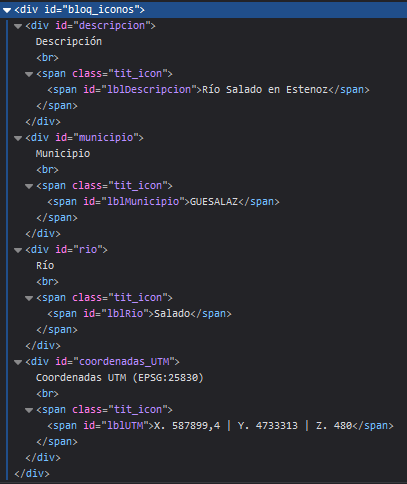
\includegraphics[width=0.7\textwidth]{fig/AguaEnNavarraEstacionHTML.png}
	\caption[HTML estación de El Agua en Navarra]{HTML estación El Agua en Navarra}
	\label{fig:ej24}
\end{figure}

Una vez se accede a los datos de la estación, se mostrara la gráfica de estos \ref{fig:ej25}. A su vez, mediante el botón "Datos Numéricos", tendremos la posibilidad de observar los datos en forma numérica. Pero no sin antes haber visitado la versión gráfica. \ref{fig:ej5}.

\begin{figure} [H]
	\centering
	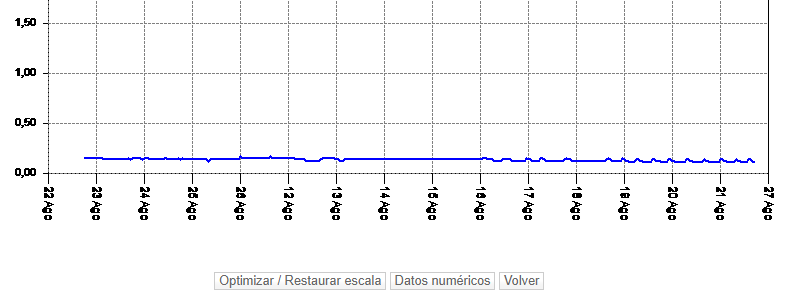
\includegraphics[width=0.7\textwidth]{fig/AguaEnNavarraGrafica.png}
	\caption[Gráfica de datos en estación de El Agua en Navarra]{Gráfica datos estación El Agua en Navarra}
	\label{fig:ej25}
\end{figure}

\begin{figure} [H]
	\centering
	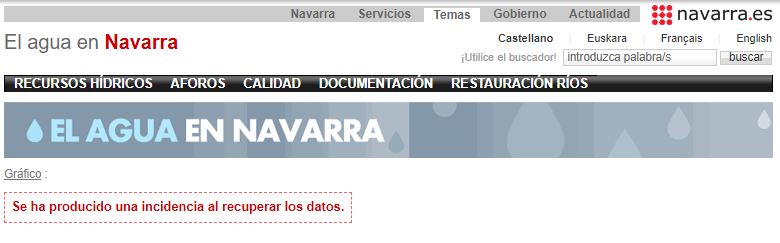
\includegraphics[width=0.7\textwidth]{fig/ErrorAguaEnNavarra.png}
	\caption[Error al cargar directamente la página de datos numéricos en El Agua en Navarra]{Error datos numéricos en El Agua en Navarra}
	\label{fig:ej5}
\end{figure}

Los datos numericos estan presentados en formato tabla cono se aprecia en la imagen \ref{fig:sub3}. Por el contrario, tras observar el HTML, realmente es un elemento div, englobando conjuntos de elementos span que representan las lineas, separados por elementos br \ref{fig:sub4}. Representando una mayor complejidad para trabajar y adquirir los datos. 

\begin{figure} [H]
	\centering
	\begin{subfigure}{.5\textwidth}
		\centering
		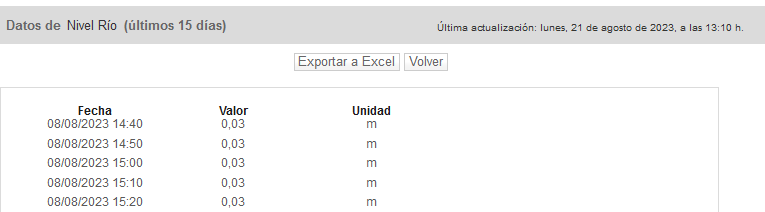
\includegraphics[width=.9\linewidth]{fig/AguaEnNavarraData.png}
		\caption{Formato presentación de los datos}
		\label{fig:sub3}
	\end{subfigure}%
	\begin{subfigure}{.5\textwidth}
		\centering
		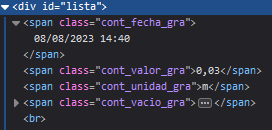
\includegraphics[width=.7\linewidth]{fig/AguaEnNavarraDataHTML.png}
		\caption{HTML de los datos}
		\label{fig:sub4}
	\end{subfigure}
	\caption{Datos numéricos de estaciones en Agua en Navarra}
	\label{fig:ej26}
\end{figure}

\section{MeteoNavarra}
En la página de meteorología y climatología de Navarra encontramos una gran sección de estaciones de las cuales poder obtener datos.
\newline
\newline
De entre los dos tipos e estaciones disponibles, automática y manual, únicamente tomamos los datos de las estaciones automáticas, esto se debe a que las manuales solo proveen datos diarios de la temperatura máxima, mínima y de la precipitación acumulada. Esto hace que no dispongamos de ningún dato hasta que finalice el día, cosa que no es viable si lo que se propone es predecir cambios radicales en un periodo de tiempo reducido.
\newline
\newline
Las estaciones automáticas proporcionan tanto datos en periodos de diez minutos como datos diarios, siguiendo el mismo razonamiento que con las estaciones manuales no tomamos los datos diarios y, entre los actualizados cada diez minutos tomamos la temperatura, humedad relativa, radiación global y precipitación en un periodo de dos días.

\begin{figure} [h!]
	\centering
	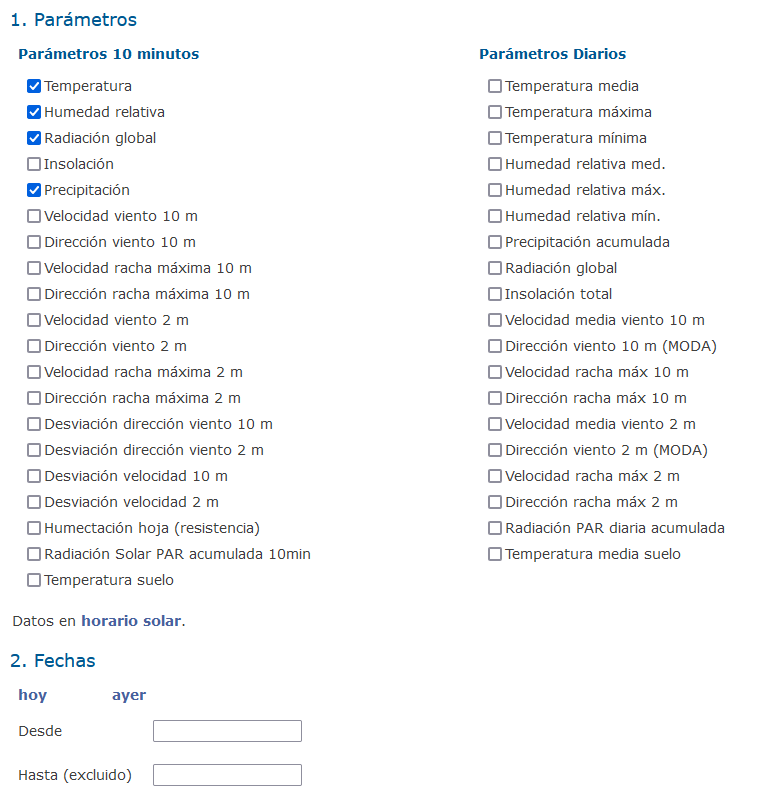
\includegraphics[width=0.7\textwidth]{fig/DatosMeteoNavarra.png}
	\caption[Apartado selección de datos MeteoNavarra]{Datos MeteoNavarra}
	\label{fig:ej6}
\end{figure}
